%%%% ijcai19.tex

\typeout{IJCAI-19 Instructions for Authors}

% These are the instructions for authors for IJCAI-19.

\documentclass{article}
\pdfpagewidth=8.5in
\pdfpageheight=11in
% The file ijcai19.sty is NOT the same than previous years'
\usepackage{ijcai19}

% Use the postscript times font!
\usepackage{times}
\usepackage{soul}
\usepackage{url}
\usepackage[hidelinks]{hyperref}
\usepackage[utf8]{inputenc}
\usepackage[small]{caption}
\usepackage{graphicx}
\usepackage{amsmath}
\usepackage{booktabs}
\usepackage{algorithm}
\usepackage{algorithmic}
\urlstyle{same}

% the following package is optional:
%\usepackage{latexsym}

% Following comment is from ijcai97-submit.tex:
% The preparation of these files was supported by Schlumberger Palo Alto
% Research, AT\&T Bell Laboratories, and Morgan Kaufmann Publishers.
% Shirley Jowell, of Morgan Kaufmann Publishers, and Peter F.
% Patel-Schneider, of AT\&T Bell Laboratories collaborated on their
% preparation.

% These instructions can be modified and used in other conferences as long
% as credit to the authors and supporting agencies is retained, this notice
% is not changed, and further modification or reuse is not restricted.
% Neither Shirley Jowell nor Peter F. Patel-Schneider can be listed as
% contacts for providing assistance without their prior permission.

% To use for other conferences, change references to files and the
% conference appropriate and use other authors, contacts, publishers, and
% organizations.
% Also change the deadline and address for returning papers and the length and
% page charge instructions.
% Put where the files are available in the appropriate places.

\title{ImageNet-trained CNNs are biased towards texture; increasing shape bias improves accuracy and robustness}

% Single author syntax
\iffalse
\author{
    Sarit Kraus
    \affiliations
    Department of Computer Science, Bar-Ilan University, Israel \emails
    pcchair@ijcai19.org
}
\fi

% Multiple author syntax (remove the single-author syntax above and the \iffalse ... \fi here)
% Check the ijcai19-multiauthor.tex file for detailed instructions

\author{
Andre Diler$^1$
\and
Mehdi Chaid$^1$\and
Abderahmane Bouziane$^1$\
\affiliations
$^1$Département GIGL Polytechnique Montreal\\
\emails
andre.diler@polymtl.ca,
mehdi.chaid@polymtl.ca,
abderahmane.bouziane@polymtl.ca
}

\begin{document}

\maketitle

\begin{abstract}
The history of computer vision led us to believe that like us, Convolutional Neural Networks (CNNs) would recognize 
objects mainly by their shapes. The paper we reproduced here introduces a novel hypothesis:
modern state of the art CNNs are more biaised towards textures than shapes. 
The autors verified their theory through multiple experiments,
and were able then to train CNNs to better recognize shapes, and surpass the state of the art models on Imagenet classification.
\end{abstract}

\section{Introduction}

% https://hackernoon.com/a-brief-history-of-computer-vision-and-convolutional-neural-networks-8fe8aacc79f3

Modern Convolutional Neural Networks reach very high performances on complex computer vision tasks like
Image classification and Image Segmentation
These performances are comparable with human perception and they come from a long history of studies.
These studies led us to believe that CNNs are shape-biased.


The first proof that edges are fundamental for vision came from a very influencal study of cognition:
  “Receptive fields of single neurons in the cat’s striate cortex”
described how biological neurons extracted features from images. It showed that certain types of
neurons were activated by edges.

The convolution of an image with a sobel filter is known to extract edges.
Other filters can extract other image features. However, the filters had to be handcrafted, and
the most significant features of an image had to be determined by a human.

Another paper showed that vision was hierachical. Low-level features (simple shapes like lines)
were combined to recognize high level features (like wheels, windows ...).

The famous Neocognition paper was the implementation of the idea of hierachical vision.
This multilayered neural network included convolutional layers with wheighted receptive fields (filters).
It was the first deep neural network.

The first modern convnet was LeNet \cite{Lecun98gradient-basedlearning}
It used backpropgation to automatically learn the filter values to extract meaningful features in images hierachically.
All the modern ConvNets are inspired from this network.

ConvNet were considered like a black box for a long time.
This is why efforts were made to analyze the internals of these networks.

The shape hypothesis is that "High-level units appear to learn
representations of shapes occurring in natural images” \cite{Kriegeskorte029876}
This hypothesis is widespread in the comunity, and
it is understandable given the history of computer vision.
There are a lot of experiments comparing human vision with computer vision.
X states that "implicitly learn representations of shape
 that reflect human shape perception".
Y said that "that  state-of-the-artone  shot  learning  models  trained  on  ImageNetexhibit  a  similar  bias  to  that  observed  in  hu-mans:  
they prefer to categorize objects according  to  shape  rather  than  color" \cite{ritter2017cognitive}

However, several studies raise doubts about this hypothesis.
According to X, CNNs are able to classify texturised images even if their shape structure is destraoyed.
Moreover, Y showed that CNNs with constrained receptive field sizes can reach competitive accuracies on ImageNet.
It is worth noticing that small receptive fields cannot capture the overal shape of an image.
These results have led the authors of the paper we reproduce \cite{geirhos2018imagenettrained} 
to emit a new hypothesis: the texture hypothesis where "in contrast to the
common assumption, object textures are more important than global object shapes for CNN object
recognition".

Our objective is to test these hypothesis with diverse experiments.

\section{Methodology}

\subsection{Intuition}


The first step of this analysis was to reproduce the original experiment of the paper with imagenette-160 
and handpicked images and textures. 
We then trained a ResNet-18 to classify the chosen images and visualize the results.
Figure 1 below shows the result of classification for a content image (a), texture image (b) and stylized image (c).

\begin{figure}[h]\centering
  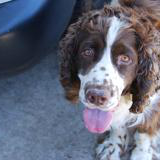
\includegraphics{imgs/dog}
  \caption*{(a) Content image: TODO GIVE NUMBERS}
\end{figure}

\begin{figure}[h]\centering
  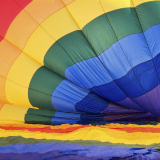
\includegraphics{imgs/texture}
  \caption*{(a) Texture image: TODO GIVE NUMBERS}
\end{figure}

\begin{figure}[h]\centering
  
\includegraphics{imgs/stylized}
  \caption*{(a) Stylized image: TODO GIVE NUMBERS}
\end{figure}

% To begin with, we reproduced the first experiment of the paper. This experiment
% is represents the misconception we have about how CNNs learn.

% Figure Mehdi

% We can see that the pretrained CNN recognized the elephant with just its texture.
% More interestingly, it recognized it classified the cat shape with elephant texture as an elephant.
% The texture hypothesis is more likely to be true.
% Let's define more robust experiments to verify that.


\subsection{Texture bias of CNNs}

General explanation

\subsubsection{IN to IN}
expected results
\subsubsection{SIN to IN}
expected results

\subsection{Dataset}

Details on dataset creation

\subsection{Resistance to noise}

Experiences Abder
Data generation

\subsection{Training}

Details of ResNet model
Hyperparams
Nb Epochs
FineTuning method

\section{Results}

\subsection{Texture bias of CNNs}

\subsection{Resistance to noise}


\section{Discussion}

\subsection{Texture bias of CNNs}

\subsection{Resistance to noise}


\appendix

%% The file named.bst is a bibliography style file for BibTeX 0.99c
\bibliographystyle{named}
\bibliography{ijcai19}

\end{document}

